%% bare_conf.tex
%% V1.3
%% 2007/01/11
%% by Michael Shell
%% See:
%% http://www.michaelshell.org/
%% for current contact information.
%%
%% This is a skeleton file demonstrating the use of IEEEtran.cls
%% (requires IEEEtran.cls version 1.7 or later) with an IEEE conference paper.
%%
%% Support sites:
%% http://www.michaelshell.org/tex/ieeetran/
%% http://www.ctan.org/tex-archive/macros/latex/contrib/IEEEtran/
%% and
%% http://www.ieee.org/

%%*************************************************************************
%% Legal Notice:
%% This code is offered as-is without any warranty either expressed or
%% implied; without even the implied warranty of MERCHANTABILITY or
%% FITNESS FOR A PARTICULAR PURPOSE! 
%% User assumes all risk.
%% In no event shall IEEE or any contributor to this code be liable for
%% any damages or losses, including, but not limited to, incidental,
%% consequential, or any other damages, resulting from the use or misuse
%% of any information contained here.
%%
%% All comments are the opinions of their respective authors and are not
%% necessarily endorsed by the IEEE.
%%
%% This work is distributed under the LaTeX Project Public License (LPPL)
%% ( http://www.latex-project.org/ ) version 1.3, and may be freely used,
%% distributed and modified. A copy of the LPPL, version 1.3, is included
%% in the base LaTeX documentation of all distributions of LaTeX released
%% 2003/12/01 or later.
%% Retain all contribution notices and credits.
%% ** Modified files should be clearly indicated as such, including  **
%% ** renaming them and changing author support contact information. **
%%
%% File list of work: IEEEtran.cls, IEEEtran_HOWTO.pdf, bare_adv.tex,
%%                    bare_conf.tex, bare_jrnl.tex, bare_jrnl_compsoc.tex
%%*************************************************************************

% *** Authors should verify (and, if needed, correct) their LaTeX system  ***
% *** with the testflow diagnostic prior to trusting their LaTeX platform ***
% *** with production work. IEEE's font choices can trigger bugs that do  ***
% *** not appear when using other class files.                            ***
% The testflow support page is at:
% http://www.michaelshell.org/tex/testflow/



% Note that the a4paper option is mainly intended so that authors in
% countries using A4 can easily print to A4 and see how their papers will
% look in print - the typesetting of the document will not typically be
% affected with changes in paper size (but the bottom and side margins will).
% Use the testflow package mentioned above to verify correct handling of
% both paper sizes by the user's LaTeX system.
%
% Also note that the "draftcls" or "draftclsnofoot", not "draft", option
% should be used if it is desired that the figures are to be displayed in
% draft mode.
%
\documentclass[10pt, conference, compsocconf]{IEEEtran}
% Add the compsocconf option for Computer Society conferences.
%
% If IEEEtran.cls has not been installed into the LaTeX system files,
% manually specify the path to it like:
%\documentclass[conference]{../sty/IEEEtran}


% Some very useful LaTeX packages include:
% (uncomment the ones you want to load)

\usepackage{subfigure}
%\usepackage{amssymb}
% *** MISC UTILITY PACKAGES ***
%
%\usepackage{ifpdf}
% Heiko Oberdiek's ifpdf.sty is very useful if you need conditional
% compilation based on whether the output is pdf or dvi.
% usage:
% \ifpdf
%   % pdf code
% \else
%   % dvi code
% \fi
% The latest version of ifpdf.sty can be obtained from:
% http://www.ctan.org/tex-archive/macros/latex/contrib/oberdiek/
% Also, note that IEEEtran.cls V1.7 and later provides a builtin
% \ifCLASSINFOpdf conditional that works the same way.
% When switching from latex to pdflatex and vice-versa, the compiler may
% have to be run twice to clear warning/error messages.






% *** CITATION PACKAGES ***
%
\usepackage{cite}
% cite.sty was written by Donald Arseneau
% V1.6 and later of IEEEtran pre-defines the format of the cite.sty package
% \cite{} output to follow that of IEEE. Loading the cite package will
% result in citation numbers being automatically sorted and properly
% "compressed/ranged". e.g., [1], [9], [2], [7], [5], [6] without using
% cite.sty will become [1], [2], [5]--[7], [9] using cite.sty. cite.sty's
% \cite will automatically add leading space, if needed. Use cite.sty's
% noadjust option (cite.sty V3.8 and later) if you want to turn this off.
% cite.sty is already installed on most LaTeX systems. Be sure and use
% version 4.0 (2003-05-27) and later if using hyperref.sty. cite.sty does
% not currently provide for hyperlinked citations.
% The latest version can be obtained at:
% http://www.ctan.org/tex-archive/macros/latex/contrib/cite/
% The documentation is contained in the cite.sty file itself.






% *** GRAPHICS RELATED PACKAGES ***
%
%\ifCLASSINFOpdf
   \usepackage[pdftex]{graphicx}
  % declare the path(s) where your graphic files are
  % \graphicspath{{../pdf/}{../jpeg/}}
  % and their extensions so you won't have to specify these with
  % every instance of \includegraphics
  % \DeclareGraphicsExtensions{.pdf,.jpeg,.png}
%\else
  % or other class option (dvipsone, dvipdf, if not using dvips). graphicx
  % will default to the driver specified in the system graphics.cfg if no
  % driver is specified.
  % \usepackage[dvips]{graphicx}
  % declare the path(s) where your graphic files are
  % \graphicspath{{../eps/}}
  % and their extensions so you won't have to specify these with
  % every instance of \includegraphics
  % \DeclareGraphicsExtensions{.eps}
%\fi
% graphicx was written by David Carlisle and Sebastian Rahtz. It is
% required if you want graphics, photos, etc. graphicx.sty is already
% installed on most LaTeX systems. The latest version and documentation can
% be obtained at: 
% http://www.ctan.org/tex-archive/macros/latex/required/graphics/
% Another good source of documentation is "Using Imported Graphics in
% LaTeX2e" by Keith Reckdahl which can be found as epslatex.ps or
% epslatex.pdf at: http://www.ctan.org/tex-archive/info/
%
% latex, and pdflatex in dvi mode, support graphics in encapsulated
% postscript (.eps) format. pdflatex in pdf mode supports graphics
% in .pdf, .jpeg, .png and .mps (metapost) formats. Users should ensure
% that all non-photo figures use a vector format (.eps, .pdf, .mps) and
% not a bitmapped formats (.jpeg, .png). IEEE frowns on bitmapped formats
% which can result in "jaggedy"/blurry rendering of lines and letters as
% well as large increases in file sizes.
%
% You can find documentation about the pdfTeX application at:
% http://www.tug.org/applications/pdftex





% *** MATH PACKAGES ***
%
\usepackage[cmex10]{amsmath}
% A popular package from the American Mathematical Society that provides
% many useful and powerful commands for dealing with mathematics. If using
% it, be sure to load this package with the cmex10 option to ensure that
% only type 1 fonts will utilized at all point sizes. Without this option,
% it is possible that some math symbols, particularly those within
% footnotes, will be rendered in bitmap form which will result in a
% document that can not be IEEE Xplore compliant!
%
% Also, note that the amsmath package sets \interdisplaylinepenalty to 10000
% thus preventing page breaks from occurring within multiline equations. Use:
%\interdisplaylinepenalty=2500
% after loading amsmath to restore such page breaks as IEEEtran.cls normally
% does. amsmath.sty is already installed on most LaTeX systems. The latest
% version and documentation can be obtained at:
% http://www.ctan.org/tex-archive/macros/latex/required/amslatex/math/





% *** SPECIALIZED LIST PACKAGES ***
%
\usepackage{algorithmic}
% algorithmic.sty was written by Peter Williams and Rogerio Brito.
% This package provides an algorithmic environment fo describing algorithms.
% You can use the algorithmic environment in-text or within a figure
% environment to provide for a floating algorithm. Do NOT use the algorithm
% floating environment provided by algorithm.sty (by the same authors) or
% algorithm2e.sty (by Christophe Fiorio) as IEEE does not use dedicated
% algorithm float types and packages that provide these will not provide
% correct IEEE style captions. The latest version and documentation of
% algorithmic.sty can be obtained at:
% http://www.ctan.org/tex-archive/macros/latex/contrib/algorithms/
% There is also a support site at:
% http://algorithms.berlios.de/index.html
% Also of interest may be the (relatively newer and more customizable)
% algorithmicx.sty package by Szasz Janos:
% http://www.ctan.org/tex-archive/macros/latex/contrib/algorithmicx/




% *** ALIGNMENT PACKAGES ***
%
%\usepackage{array}
% Frank Mittelbach's and David Carlisle's array.sty patches and improves
% the standard LaTeX2e array and tabular environments to provide better
% appearance and additional user controls. As the default LaTeX2e table
% generation code is lacking to the point of almost being broken with
% respect to the quality of the end results, all users are strongly
% advised to use an enhanced (at the very least that provided by array.sty)
% set of table tools. array.sty is already installed on most systems. The
% latest version and documentation can be obtained at:
% http://www.ctan.org/tex-archive/macros/latex/required/tools/


%\usepackage{mdwmath}
%\usepackage{mdwtab}
% Also highly recommended is Mark Wooding's extremely powerful MDW tools,
% especially mdwmath.sty and mdwtab.sty which are used to format equations
% and tables, respectively. The MDWtools set is already installed on most
% LaTeX systems. The lastest version and documentation is available at:
% http://www.ctan.org/tex-archive/macros/latex/contrib/mdwtools/


% IEEEtran contains the IEEEeqnarray family of commands that can be used to
% generate multiline equations as well as matrices, tables, etc., of high
% quality.


%\usepackage{eqparbox}
% Also of notable interest is Scott Pakin's eqparbox package for creating
% (automatically sized) equal width boxes - aka "natural width parboxes".
% Available at:
% http://www.ctan.org/tex-archive/macros/latex/contrib/eqparbox/





% *** SUBFIGURE PACKAGES ***
%\usepackage[tight,footnotesize]{subfigure}
% subfigure.sty was written by Steven Douglas Cochran. This package makes it
% easy to put subfigures in your figures. e.g., "Figure 1a and 1b". For IEEE
% work, it is a good idea to load it with the tight package option to reduce
% the amount of white space around the subfigures. subfigure.sty is already
% installed on most LaTeX systems. The latest version and documentation can
% be obtained at:
% http://www.ctan.org/tex-archive/obsolete/macros/latex/contrib/subfigure/
% subfigure.sty has been superceeded by subfig.sty.



%\usepackage[caption=false]{caption}
%\usepackage[font=footnotesize]{subfig}
% subfig.sty, also written by Steven Douglas Cochran, is the modern
% replacement for subfigure.sty. However, subfig.sty requires and
% automatically loads Axel Sommerfeldt's caption.sty which will override
% IEEEtran.cls handling of captions and this will result in nonIEEE style
% figure/table captions. To prevent this problem, be sure and preload
% caption.sty with its "caption=false" package option. This is will preserve
% IEEEtran.cls handing of captions. Version 1.3 (2005/06/28) and later 
% (recommended due to many improvements over 1.2) of subfig.sty supports
% the caption=false option directly:
%\usepackage[caption=false,font=footnotesize]{subfig}
%
% The latest version and documentation can be obtained at:
% http://www.ctan.org/tex-archive/macros/latex/contrib/subfig/
% The latest version and documentation of caption.sty can be obtained at:
% http://www.ctan.org/tex-archive/macros/latex/contrib/caption/




% *** FLOAT PACKAGES ***
%
%\usepackage{fixltx2e}
% fixltx2e, the successor to the earlier fix2col.sty, was written by
% Frank Mittelbach and David Carlisle. This package corrects a few problems
% in the LaTeX2e kernel, the most notable of which is that in current
% LaTeX2e releases, the ordering of single and double column floats is not
% guaranteed to be preserved. Thus, an unpatched LaTeX2e can allow a
% single column figure to be placed prior to an earlier double column
% figure. The latest version and documentation can be found at:
% http://www.ctan.org/tex-archive/macros/latex/base/



%\usepackage{stfloats}
% stfloats.sty was written by Sigitas Tolusis. This package gives LaTeX2e
% the ability to do double column floats at the bottom of the page as well
% as the top. (e.g., "\begin{figure*}[!b]" is not normally possible in
% LaTeX2e). It also provides a command:
%\fnbelowfloat
% to enable the placement of footnotes below bottom floats (the standard
% LaTeX2e kernel puts them above bottom floats). This is an invasive package
% which rewrites many portions of the LaTeX2e float routines. It may not work
% with other packages that modify the LaTeX2e float routines. The latest
% version and documentation can be obtained at:
% http://www.ctan.org/tex-archive/macros/latex/contrib/sttools/
% Documentation is contained in the stfloats.sty comments as well as in the
% presfull.pdf file. Do not use the stfloats baselinefloat ability as IEEE
% does not allow \baselineskip to stretch. Authors submitting work to the
% IEEE should note that IEEE rarely uses double column equations and
% that authors should try to avoid such use. Do not be tempted to use the
% cuted.sty or midfloat.sty packages (also by Sigitas Tolusis) as IEEE does
% not format its papers in such ways.





% *** PDF, URL AND HYPERLINK PACKAGES ***
%
\usepackage{url}
% url.sty was written by Donald Arseneau. It provides better support for
% handling and breaking URLs. url.sty is already installed on most LaTeX
% systems. The latest version can be obtained at:
% http://www.ctan.org/tex-archive/macros/latex/contrib/misc/
% Read the url.sty source comments for usage information. Basically,
% \url{my_url_here}.





% *** Do not adjust lengths that control margins, column widths, etc. ***
% *** Do not use packages that alter fonts (such as pslatex).         ***
% There should be no need to do such things with IEEEtran.cls V1.6 and later.
% (Unless specifically asked to do so by the journal or conference you plan
% to submit to, of course. )


% correct bad hyphenation here
\begin{document}
% paper title
% can use linebreaks \\ within to get better formatting as desired
\title{ \textbf{C}lassification of \textbf{C}rowdsourced \textbf{T}ext \textbf{C}orrection}


% author names and affiliations
% use a multiple column layout for up to two different
% affiliations

\author{\IEEEauthorblockN{Haimonti Dutta \thanks{The author is also an adjunct assistant professor at IIIT, Delhi.}
\IEEEauthorblockA{Institute of Data Sciences and Engineering (IDSE),\\
Columbia University\\
New York, NY 10115\\
hd2200columbia@gmail.com}\\
\and
\IEEEauthorblockN{Megha Gupta}
\IEEEauthorblockA{Dept. of Computer Science\\
IIIT-Delhi, India.\\
meghag@iiitd.ac.in}
\and 
\IEEEauthorblockN{Brian Geiger}
Center for Bibliographical Studies\\
and Research\\
University of California, Riverside.\\
brian.geiger@ucr.edu
}
}


% conference papers do not typically use \thanks and this command
% is locked out in conference mode. If really needed, such as for
% the acknowledgment of grants, issue a \IEEEoverridecommandlockouts
% after \documentclass

% for over three affiliations, or if they all won't fit within the width
% of the page, use this alternative format:
% 
%\author{\IEEEauthorblockN{Michael Shell\IEEEauthorrefmark{1},
%Homer Simpson\IEEEauthorrefmark{2},
%James Kirk\IEEEauthorrefmark{3}, 
%Montgomery Scott\IEEEauthorrefmark{3} and
%Eldon Tyrell\IEEEauthorrefmark{4}}
%\IEEEauthorblockA{\IEEEauthorrefmark{1}School of Electrical and Computer Engineering\\
%Georgia Institute of Technology,
%Atlanta, Georgia 30332--0250\\ Email: see http://www.michaelshell.org/contact.html}
%\IEEEauthorblockA{\IEEEauthorrefmark{2}Twentieth Century Fox, Springfield, USA\\
%Email: homer@thesimpsons.com}
%\IEEEauthorblockA{\IEEEauthorrefmark{3}Starfleet Academy, San Francisco, California 96678-2391\\
%Telephone: (800) 555--1212, Fax: (888) 555--1212}
%\IEEEauthorblockA{\IEEEauthorrefmark{4}Tyrell Inc., 123 Replicant Street, Los Angeles, California 90210--4321}}




% use for special paper notices
%\IEEEspecialpapernotice{(Invited Paper)}




% make the title area
\maketitle

\begin{abstract}
Optical Character Recognition (OCR) is a commonly used technique for digitizing printed material enabling them to be displayed online, searched and used in text mining applications. 
The text generated from OCR devices is often garbled due to variations in quality of the input paper, size and style of the font and column layout. This adversely affects retrieval effectiveness and hence techniques for cleaning the garbled text need to be improvised. Often such techniques involve laborious and time consuming manual processing of data. This paper presents a prototype system for \textbf{C}lassification of \textbf{C}rowdsourced \textbf{T}ext \textbf{C}orrection (CCTC) which takes as input log files containing garbled and manually corrected OCR text, parses and tokenizes them and builds models for categorizing the corrections using state-of-the-art machine learning algorithms. Retrieval effectiveness on the California Digital Newspaper Collection is measured using mean reciprocal rank. 
This prototype system is expected to be deployed on historical newspaper archives that make extensive use of user text corrections.
\end{abstract}

%\begin{IEEEkeywords}
%component; formatting; style; styling;
%
%\end{IEEEkeywords}


% For peer review papers, you can put extra information on the cover
% page as needed:
% \ifCLASSOPTIONpeerreview
% \begin{center} \bfseries EDICS Category: 3-BBND \end{center}
% \fi
%
% For peerreview papers, this IEEEtran command inserts a page break and
% creates the second title. It will be ignored for other modes.
\IEEEpeerreviewmaketitle



\section{Introduction}
\label{sec:intro}

Crowdsourcing is used extensively in cultural heritage and digital history related projects in recent years to digitize, create and process content and provide editorial or processing interventions. For example, the Australian Newspapers Digitization Program \cite{ADNP} allows communities to explore their rich newspaper heritage by enabling free online public access to over 830,000 newspaper pages containing 8.4 million articles. The public enhanced the data by correcting over 7 million lines of text and adding 200,000 tags and 4600 comments \cite{holley_09}. 
%Picture Australia \cite{pictAus} harvests digital images from other heritage institutions and encourages the public to upload their own images and tag them. 
FamilySearch \cite{famSearch} made available handwritten digital images of births, deaths and marriage records for transcription by the public. The New York Public Library has 1,277,616 dishes transcribed to date from 17,079 menus. 
%Galaxy Zoo \cite{galZoo} is an online collaborative astronomy project in which users are invited to classify millions of galaxies from digital photos. 

In all of the above crowdsourcing projects, large volumes of data are generated by users. These include tags, folksonomies, flagged content, information on history, relationship and preference data, structured labels describing objects and creative responses \cite{Ridge_11}. However, little statistical analysis is done of the user generated content in most cases. Assessment of data quality obtained by leveraging the ``wisdom of the crowd" remains an open problem. 

%Before this question can be answered, statistical analysis of the data generated is imperative.

In this paper, we focus on understanding the nature of text corrections done by users of an old historic newspaper archive. The newspapers are made available for searching on the Internet after the following processes take place: (1) the microfilm copy or paper original is scanned; %(2) master and Web image files are generated; 
(2) metadata is assigned for each page to improve the search capability of the newspaper; (3) OCR software is run over high resolution images to create searchable full text.
% and (5) OCR text, images, and metadata are imported into a digital library software program. 
The OCR scanning process is far from perfect and the documents generated from it contains a large amount of garbled text. A user is presented with a high resolution image of a newspaper page along with erroneous or distorted text from the OCR and is expected to rectify the garbled words as appropriate. A prototype for a system that can be used for \textbf{C}lassification of \textbf{C}rowdsourced \textbf{T}ext \textbf{C}orrection (CCTC) is presented which can answer simple questions such as ``What are the different kinds corrections proposed by users?" and provide statistics generated from the correction process. The output from the system can be used to enhance search and retrieval.

The study used log files generated from text correction software in use at the California Digital Newspaper Collection (CDNC)\footnote{http://cdnc.ucr.edu/cgi-bin/cdnc}, which contains over 400,000 pages of newspapers published in California between 1846-1922. 
%To date, the archive has approximately 1680 registered users who have corrected close to 2 million lines of text. 
%The corrections are primarily categorized as changes in spellings, punctuation rectification, addition of content or capitalization. A semi-automatic engine for classifying corrections based on support vector machines is designed.  
To the best of our knowledge, this is the first attempt to statistically analyze and model OCR error corrections provided by the crowd. We posit that such a classification system will be beneficial when attempting to compensate the annotators; it can also be used for task allocation if some users are more comfortable with certain type of corrections than others.

%In a bid to serve its patrons better, the CDNC crowdsourced the cleaning of OCR text. To date..
\begin{figure*}[t]
\centering
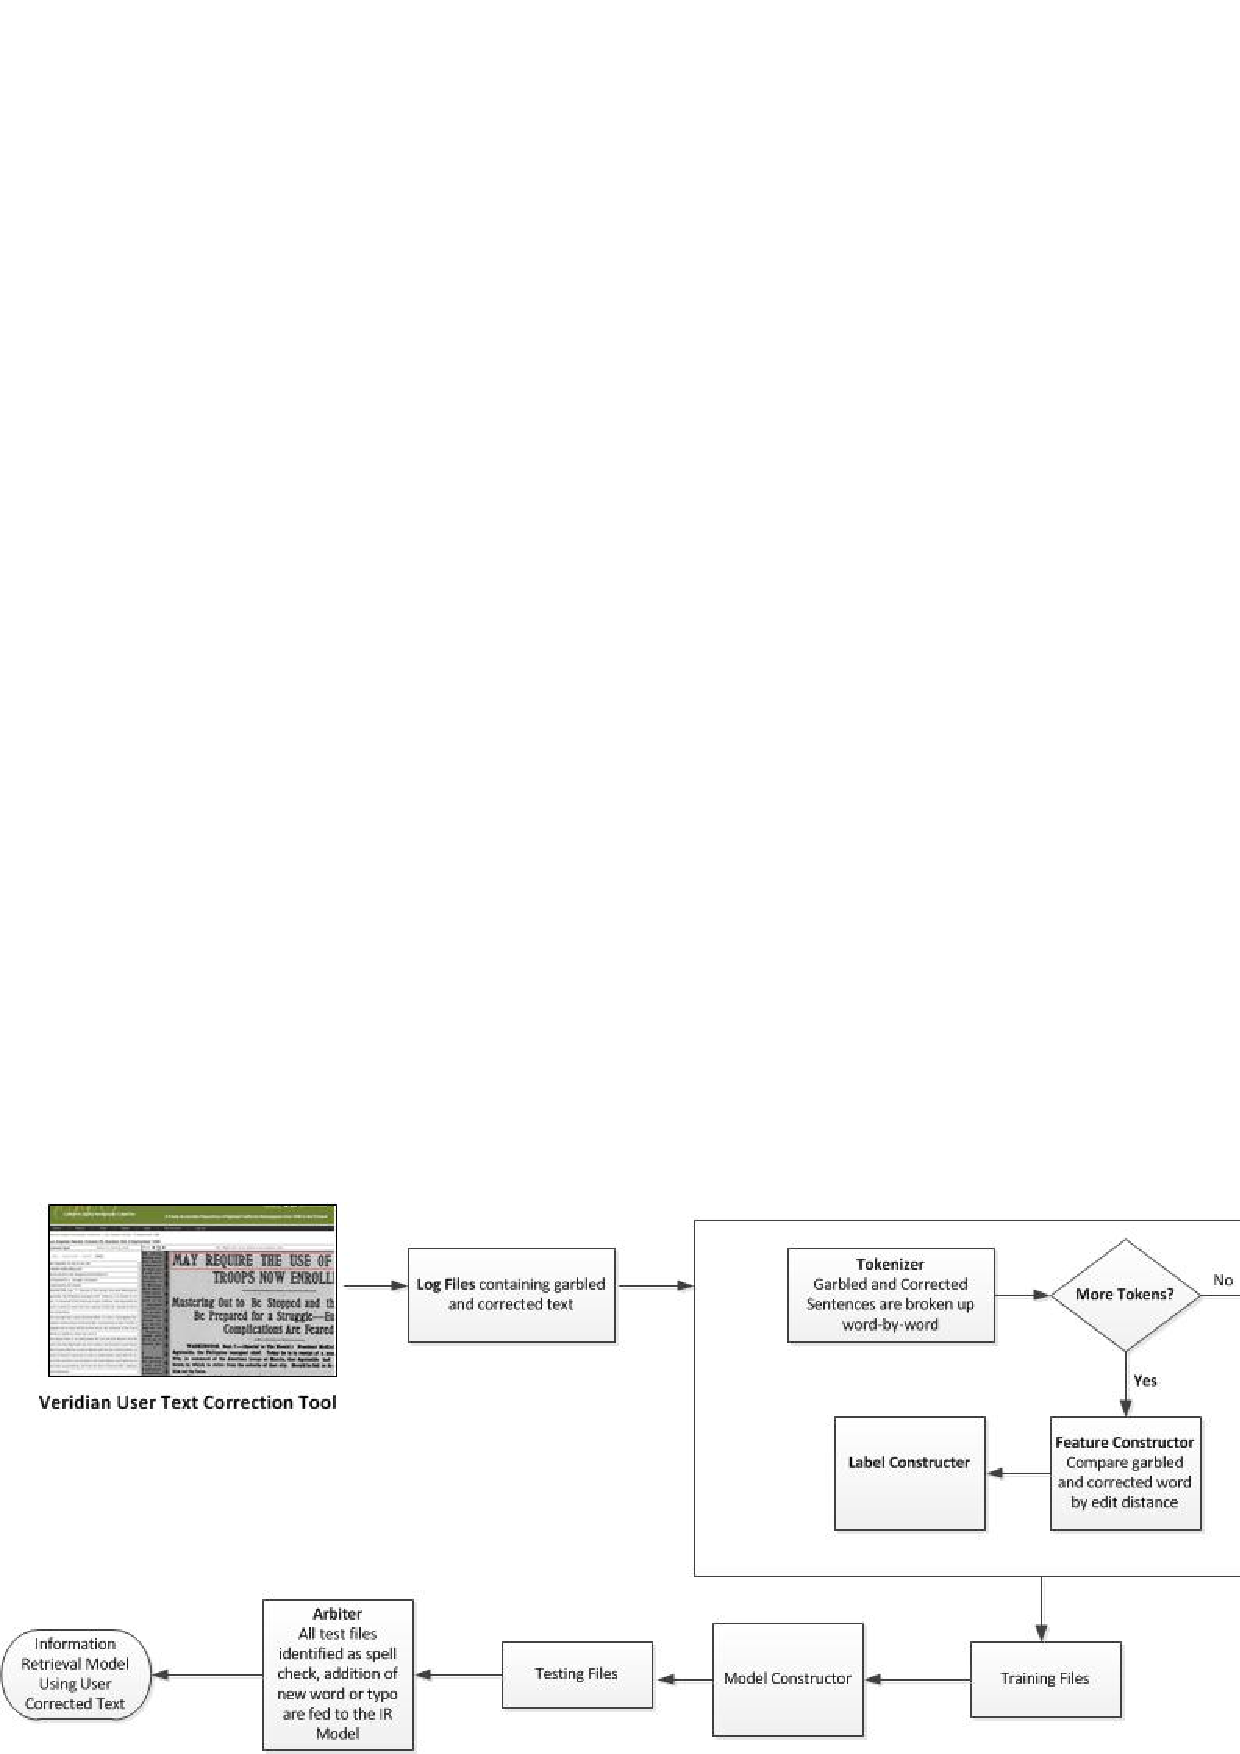
\includegraphics[width=0.8\textheight]{./image/archOCR.jpg}
\caption{The Architecture of the Proposed System}
\label{fig:arch}
\end{figure*}

\noindent \textbf{Organization}: Section~\ref{arch} describes the architecture of the proposed system; Section~\ref{sec:evaluation} presents empirical and scalability results on real-world data collected at CDNC; Section~\ref{ir} presents information retrieval techniques; Section~\ref{sec:related} discusses related work. Finally, Section~\ref{sec:conc} concludes the paper.

\section{Architecture of the Proposed System}
\label{arch}
The \textbf{C}lassification of \textbf{C}rowdsourced \textbf{T}ext \textbf{C}orrection (CCTC) system has the following components:

\begin{enumerate}

\item The \textbf{Veridian User Text Correction}\footnote{http://veridiansoftware.com/crowdsourcing/} tool which takes as input a scanned page of the newspaper and enables users to correct OCR errors as they come across them.
Figure~\ref{fig:T1} shows an example of a scanned page from ``The Amador Ledger" published on January 26, 1900. The article to be corrected by a user is highlighted. The raw OCR text from the article and the tool used by patrons to correct text is shown in figure ~\ref{fig:T2}.


\item \textbf{Log Files: }All corrections performed by the annotators are recorded in log files. To date approximately 1,705,149 lines have been edited by 848 annotators which resulted in 235 log files. A sample of 191 files has been used for this work. Each log file is generated at the issue-level and contains XML data about the pages in the issue. Table~\ref{table:logfile} describes the structure of the log file. The following information is provided about the corrections made by the patrons:
%\begin{enumerate}
(a) \textit{Page Id: } The id of the page in which editing was done.
(b) \textit{Block Id: } The id of the paragraph containing the line corrected by the user.
(c) \textit{Line Id: }The id of the line edited by the user.
(d) \textit{Old Text Value} is the garbled text generated by the OCR device and replaced by the user.
(e) \textit{New Text Value} is the corrected text with which the old text was replaced.
%\end{enumerate}

\begin{table}[h]
\begin{center}
\begin{tabular}{l}
\textless TextCorrectedLine lineID="P2\_TL00800"\textgreater \\
\textless OldTextValue\textgreater \textbf{Spll, Stales}\textless /OldTextValue\textgreater \\
\textless NewTextValue\textgreater \textbf{Union Stables}\textless /NewTextValue\textgreater \\
\textless /TextCorrectedLine\textgreater \\
\textless TextCorrectedLine lineID="P2\_TL00801"\textgreater \\
\textless OldTextValue\textgreater \textbf{**?�** Under Webb Hall *}\textless/OldTextValue\textgreater \\
\textless NewTextValue\textgreater \textbf{Under Webb Hall} \textless/NewTextValue\textgreater \\
\textless /TextCorrectedLine\textgreater \\
\end{tabular}
\end{center}
\caption{A segment of the log file}
\label{table:logfile}
\end{table}

\begin{figure*}[ht]
\begin{center}
%\mbox{
\subfigure[Scanned newspaper highlighting an article to be corrected by a user.]
{
%%\includegraphics[width=0.6\columnwidth]{odds_20070813_160000rb_M.pdf}
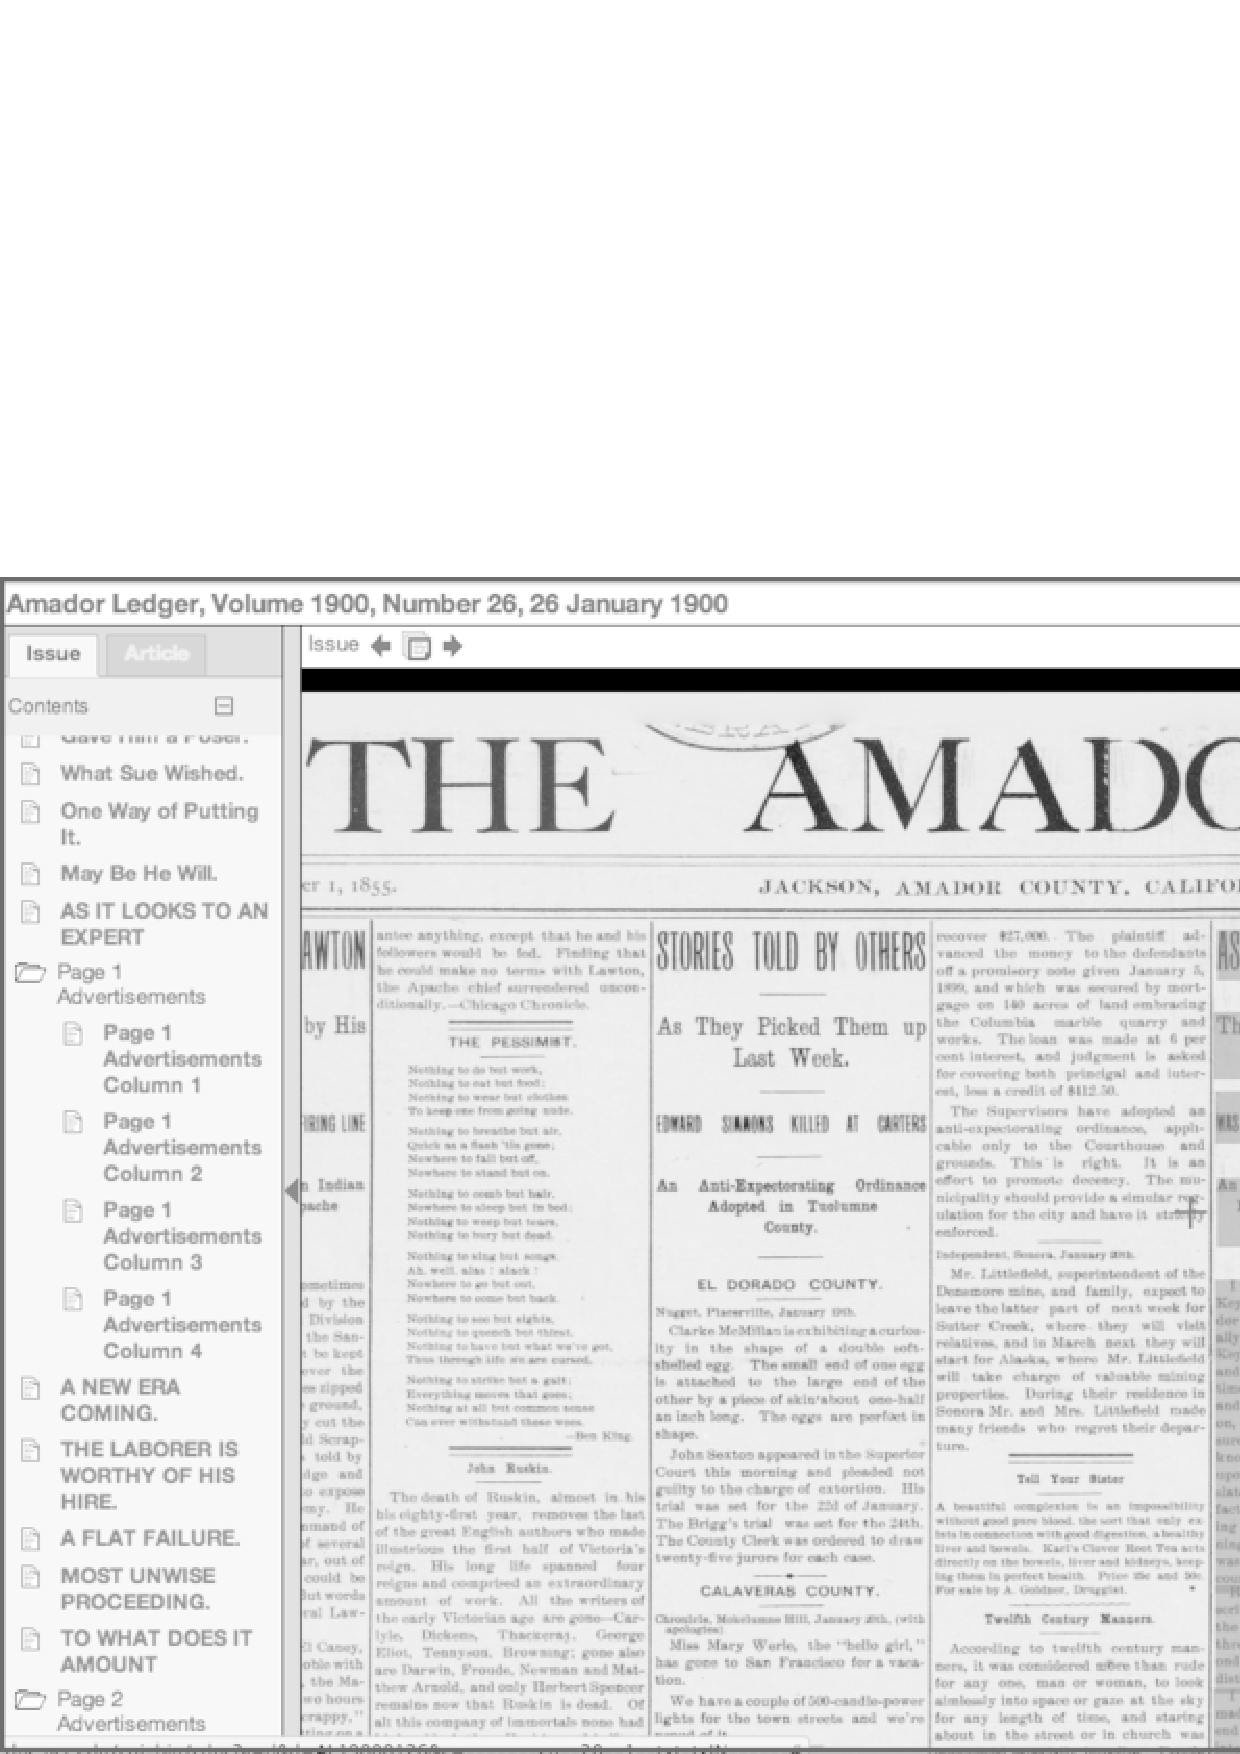
\includegraphics[width=0.48\textwidth, height=0.2\textheight]{./image/greyscale.jpg}
\label{fig:T1}
}
\subfigure[The tool used by patrons to annotate articles.]
{
%%\includegraphics[width=0.8\columnwidth]{20070813-C1-7d-roc.pdf}
\includegraphics[width=0.48\textwidth,height=0.2\textheight]{./image/correction.jpg}
\label{fig:T2}
}
\caption{The Amador Ledger, Jan. 26, 1900.}
\label{News_01}
\end{center}
\end{figure*}

\item \textbf{Preprocessor: } The preprocessor has three main components:
\begin{itemize}
\item \textbf{Tokenizer: } The old text and the corresponding new text from the log file is tokenized by white-spaces. There are 44,022 tokens of which 21,108 are corrected by the annotators.

\item \textbf{Feature Constructor: } Features are crafted by computing the Levenshtein edit distance between the old word and its correction. The Levenshtein edit distance \cite{Wagner_74} is defined as the minimum number of single edit operations (insertions, deletions and substitutions) required to convert one string into another. Six binary features are generated as follows: 
(a) \textbf{Difference Length Zero} : $1$, if both the old word and new word have same length and $0$ otherwise. 
%For example, the feature is 1 for the tokens ``Spll," and ``Union" as  both the tokens have same number of characters.
(b) \textbf{Difference Length Above One} : $1$, if the length of new word exceeds the length of old word and $0$ otherwise.
(c) \textbf{Edit Distance One}:  $1$, if single edit operation is required to convert old word to new word and $0$ otherwise. For example, the feature is 1 for tokens ``Under" and ``under" or ``the" and ``them".
(d) \textbf{Edit Distance Above One}: $1$, if more than one edit operation is required to convert old word to new word and $0$ otherwise. For ``Spll," and ``Union", value is 1 as more than one edit operation is required to convert from old to new token.
%(d) \textbf{Edit Distance Below Three}: 1, if less than three edit operations are required to convert old word to new word and $0$ otherwise. 
%For ``Stales" and ``Stables", value is 1 as less than three edit operations are required to convert from old to new token. 
(e) \textbf{Edit Distance is 1 and Case Change}: 1, if the two words have edit distance is exactly 1 and the first character of one string change from upper case to lower case or vice versa. For example, for ``Stales" and ``Stables", the value is 0 as there is no case change.
(f) \textbf{Punctuation Difference}: 1, if both the old text and new text differ in any of the following punctuation marks (!"\#\$\%\&'*+,-./:;\textless=\textgreater?@[$\backslash$]\^\_`\{\textbar\}\textasciitilde).


%\begin{figure*}[t]
%\centering
%\includegraphics[width=0.9\textwidth]{./image/flowchartnew.jpg}
%%\includegraphics[width=6cm,height=4cm]{./image/error.jpg}
%\caption{Flowchart demonstrating how the labels are generated.}
%\label{fig:flowchart}
%\end{figure*}

\item \textbf{Label Constructor: }The errors rectified by the users are categorized as addition, deletion, punctuation error, capitalization error, and spellcheck error. 
%The logic used in generation of the features can be summarized by the flowchart depicted in Figure~\ref{fig:flowchart}.
Specifically,
%\begin{enumerate}
(a) \textbf{Addition: } When the length of new string exceeds the length of old given the difference is made by alphanumeric characters and the edit distance is above one. For example, ``6RAVR" and ``GRAVEL".
(b) \textbf{Deletion: }When the length of old string exceeds the length of new given the difference is made by alphanumeric characters and the edit distance is above one. For example, ``VVe" and ``We".
(c) \textbf{Punctuation: }When the difference in the length of strings is non-zero and they differ by special characters contained in the set (!"\#\$\%\&'()*+,-./:;\textless=\textgreater?@[$\backslash$]\^\_`\{\textbar\}\textasciitilde). For example, ``Ladies!" and ``Ladies".
(d) \textbf{Capitalization: }When both the strings have equal length, edit distance is exactly 1 and first letter of both the strings change from upper to lower case or vice versa. For example, ``largest" and ``Largest".
(e) \textbf{Spellcheck: }When the difference between string is above zero and the edit distance contributed by alphanumeric character is exactly one or when the strings have same length and the edit distance is one or above one irrespective of the involvement of special characters. For example, ``the" and ``them" or ``hanger" and ``banger".

%(a)\textbf{Spellcheck Error: }When the edit distance is between 1 and 3. For example, ``mounten" and ``mountain".
%(b)\textbf{Addition of a new word: }When the edit distance is more than 3. For example, ``at" and ``attend".
%(c)\textbf{Capitalization error: } When the edit distance of two strings is exactly 1 and first letter of both the strings changes from upper to lower case or vice versa. For example, ``largest" and ``Largest".
%(d)\textbf{Typographical Error: } When the edit distance is exactly one and case change is 0. For example, ``teh" and ``the"
%(e)\textbf{Punctuation Error: }When the two strings differ by special characters contained in the set (!"\#\$\%\&'()*+,-./:;\textless=\textgreater?@[$\backslash$]\^\_`\{\textbar\}\textasciitilde). 
%%For example, ``residents" and residents
%(f)\textbf{No Correction: }When the old and new text are same. %For example, plant and plant
%%\end{enumerate}

The distribution of the these classes in the dataset is shown in Table~\ref{table: classes}. It must be noted that by design tokens are always assigned to one class, although in principle it may be possible to assign them to multiple classes\footnote{For e.g. a correction of ``t$\$$e" to ``the" could be either a Spellcheck or a Punctuation Error correction but we assign it to Spellcheck }.

\begin{table}[htdp]
\begin{center}
\begin{tabular}{| l | l |}
\hline
 Class  & No. of Instances \\
\hline
 Addition & 4575 \\
%\hline 
Deletion & 5024 \\
%\hline
Punctuation & 6401 \\
%\hline
Capitalization & 299 \\
%\hline
Spellcheck & 4809 \\
%\aline 
\hline
Total & 21108 \\
\hline
\end{tabular}
\end{center}
\caption{Class Distribution}
\label{table: classes}
\end{table}

\end{itemize}

%\begin{figure}[h]
%\centering
%\includegraphics[width=0.48\textwidth]{./image/error.jpg}
%%\includegraphics[width=6cm,height=4cm]{./image/error.jpg}
%\caption{Error Classification}
%\label{fig:stats}
%\end{figure}

%The dataset was parsed to a format used by the Joachim's multi class SVM algorithm which is represented as\\
%\textless target\textgreater\space\textless feature\textgreater:\textless value\textgreater ......\textless feature\textgreater:\textless value\textgreater\\
%The number of instances in the dataset is 44,022. 
%The class distribution in the dataset is shown in table ~\ref{table: classes}

\item \textbf{Baseline Character-Level Feature Construction: }
The tokenization process of the text in the log files was modified to enable the addition and deletion classification of text using a character. If the text was deleted by the user as a part of correction process then the character ``$\sim$" was assigned to the new token denoting that the user performed the task of deleting the OCR garbled text whereas if the user added a new text  then the character ``+" was assigned to the old token denoting that user added text that was initially missing in the OCR data. All the corrected tokens were further split into character level data with the tuple \textless old char, new char\textgreater  replacing the previous token level notion of \textless old token,new token\textgreater giving us $58,963$ instances of data. Of $58,963$ instances, we encountered that $55,612$ instances were redundant which signifies that the OCR device makes the same type of mistakes repeatedly. The maximum number of redundant corrections noted were deletion of punctuations and special characters. There were $4344$ deletions of comma, $2831$ deletions of $\ddot{A}$. Amongst character to character corrections, $635$ cases of o$\rightarrow$e, $470$ cases of b$\rightarrow$h, 299 cases of u$\rightarrow$n contributed maximum to the redundancy. Hence, the number of unique instances was found to be $3351$. Figure ~\ref{fig:stat1}, ~\ref{fig:stat2} shows histograms where examples of few o$\rightarrow$e and b$\rightarrow$h corrections have taken place. In order to test the performance of the manually crafted features of the dataset, we automatically generated rules using apriori algorithm to mine association rules. Mining association rules means to find all association rules that have support and confidence greater than or equal to user specified minimum support ($minsup$) and minimum confidence ($minconf$) respectively. In our case, the value of $minconf$ and the the lower bound $minsup$ was set to $0.0001$, and the upper bound of $minsup$ was set to $1$. The upper bound of $minsup$ was iteratively decreased by a factor of $delta$ until either the lower bound of $minsup$ was reached or the required number of rules were generated. The number of rules generated by the algorithm were $6631$.
%Some of the user defined parameters used in the algorithm are support and confidence. Support, sup(o$\rightarrow$e) is defined as the probability that letter `o' gets replaced to letter `e'. And confidence, conf(o$\rightarrow$e) is defined as the probability that the new character is `e' given the old character is `o'.
%minimum confidence, was set to 1.0E-4, delta:  1.0E-4, upper bound minimum support: 1.0, lower bound minimum support: 1.0E-4.



The error labels are the same as that for token level data.
(a) \textbf{Addition: } When a user inserts a new token `T' in place of void, the old character is assigned a symbol `+'. For example, + $\rightarrow$ T.
(b) \textbf{Deletion: } When a user removes an existing token `A' from the old text, the new character is assigned a symbol `$\sim$'. For example, A $\rightarrow$ $\sim$.
(c) \textbf{Capitalization error: } When an old character is capitalized or decapitalized to form a new character. For example, l $\rightarrow$ L.
(d) \textbf{Punctuation error: } When a substitution of an old to new character involves a punctuation. For example, ! $\rightarrow$ t.
(e) \textbf{Spellcheck error: } When an old alphanumeric character is replaced by a new alphanumeric character. For example, o $\rightarrow$ e.

\begin{figure*}[ht]
\begin{center}
%\mbox{
\subfigure[o changed to e]
{
%%\includegraphics[width=0.8\columnwidth]{20070813-C1-7d-roc.pdf}
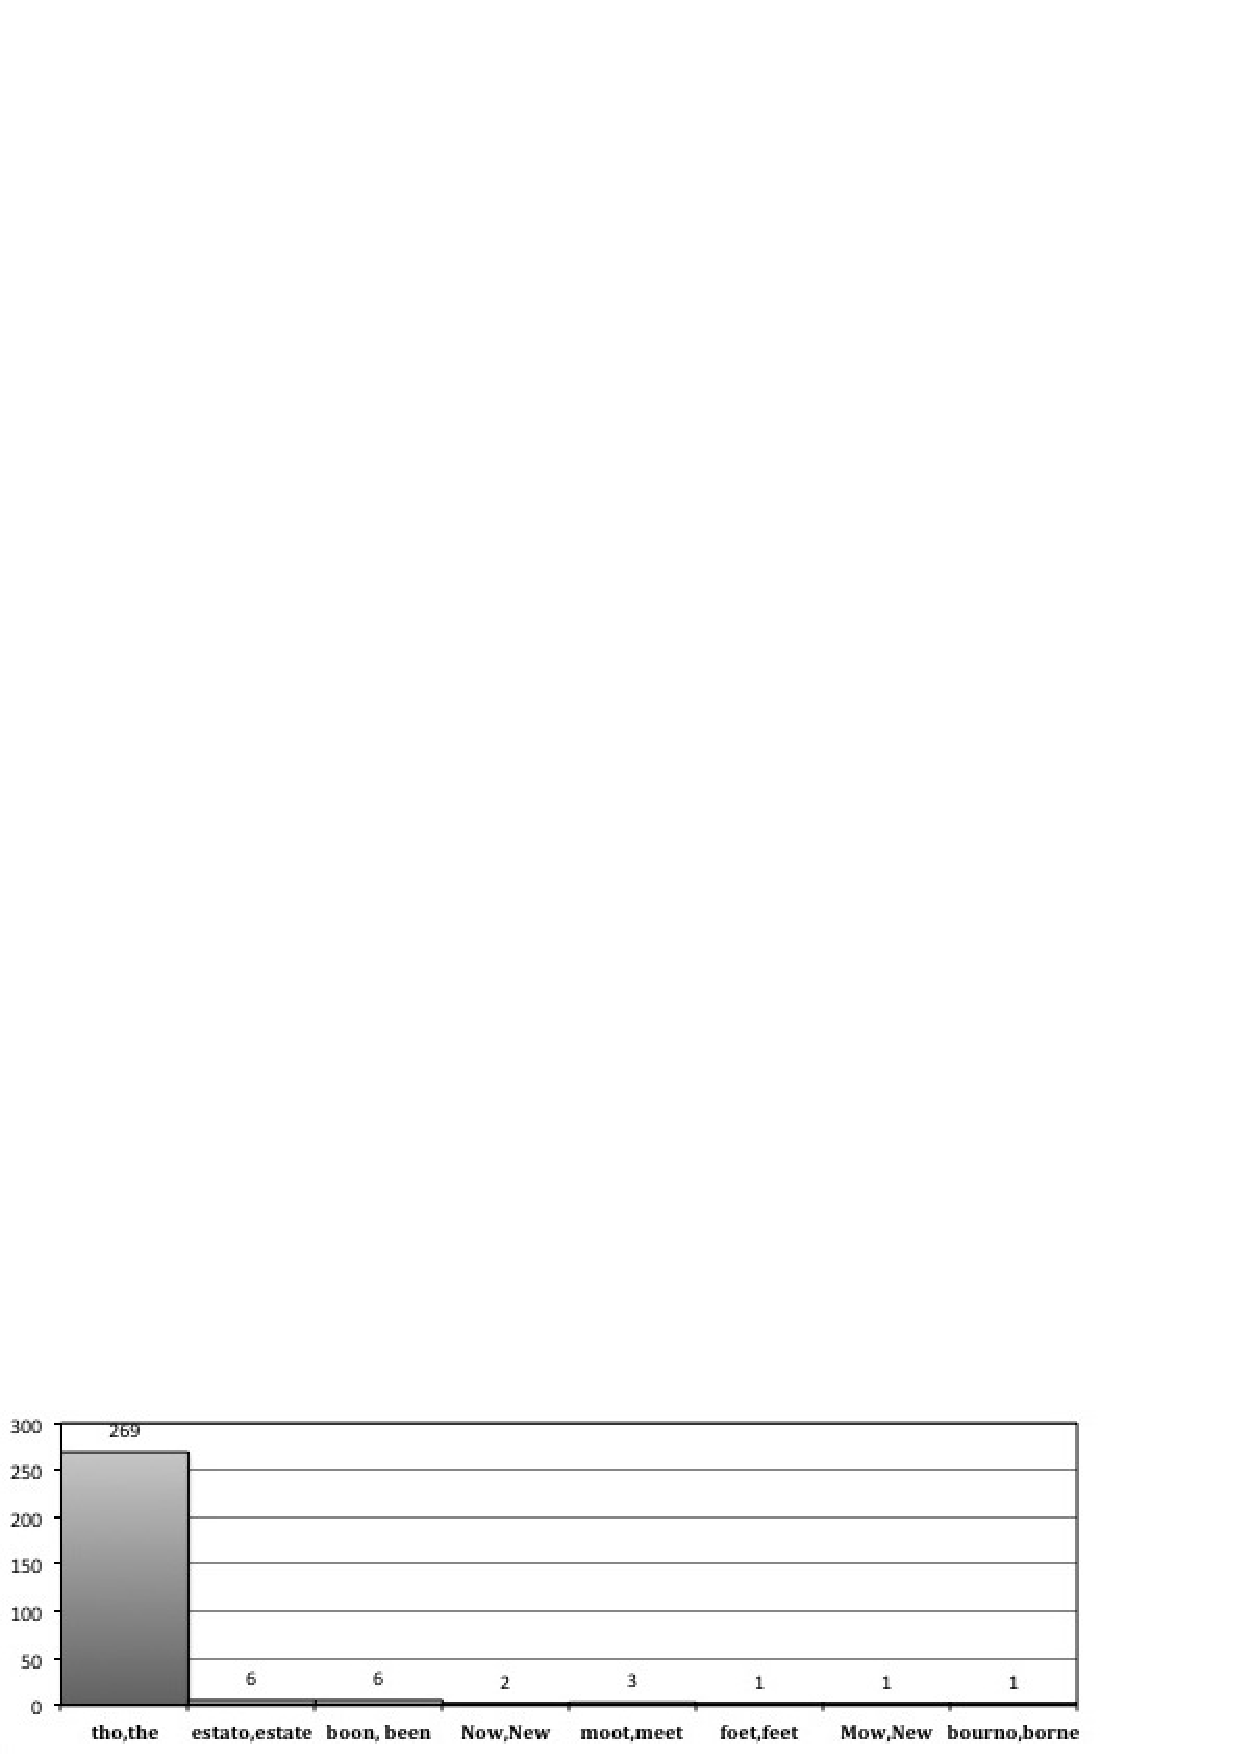
\includegraphics[width=0.45\textwidth, height=0.13\textheight]{./image/stat1edit.jpg}
\label{fig:stat1}
}
\subfigure[b changed to h]
{
%%\includegraphics[width=0.8\columnwidth]{20070813-C1-7d-roc.pdf}
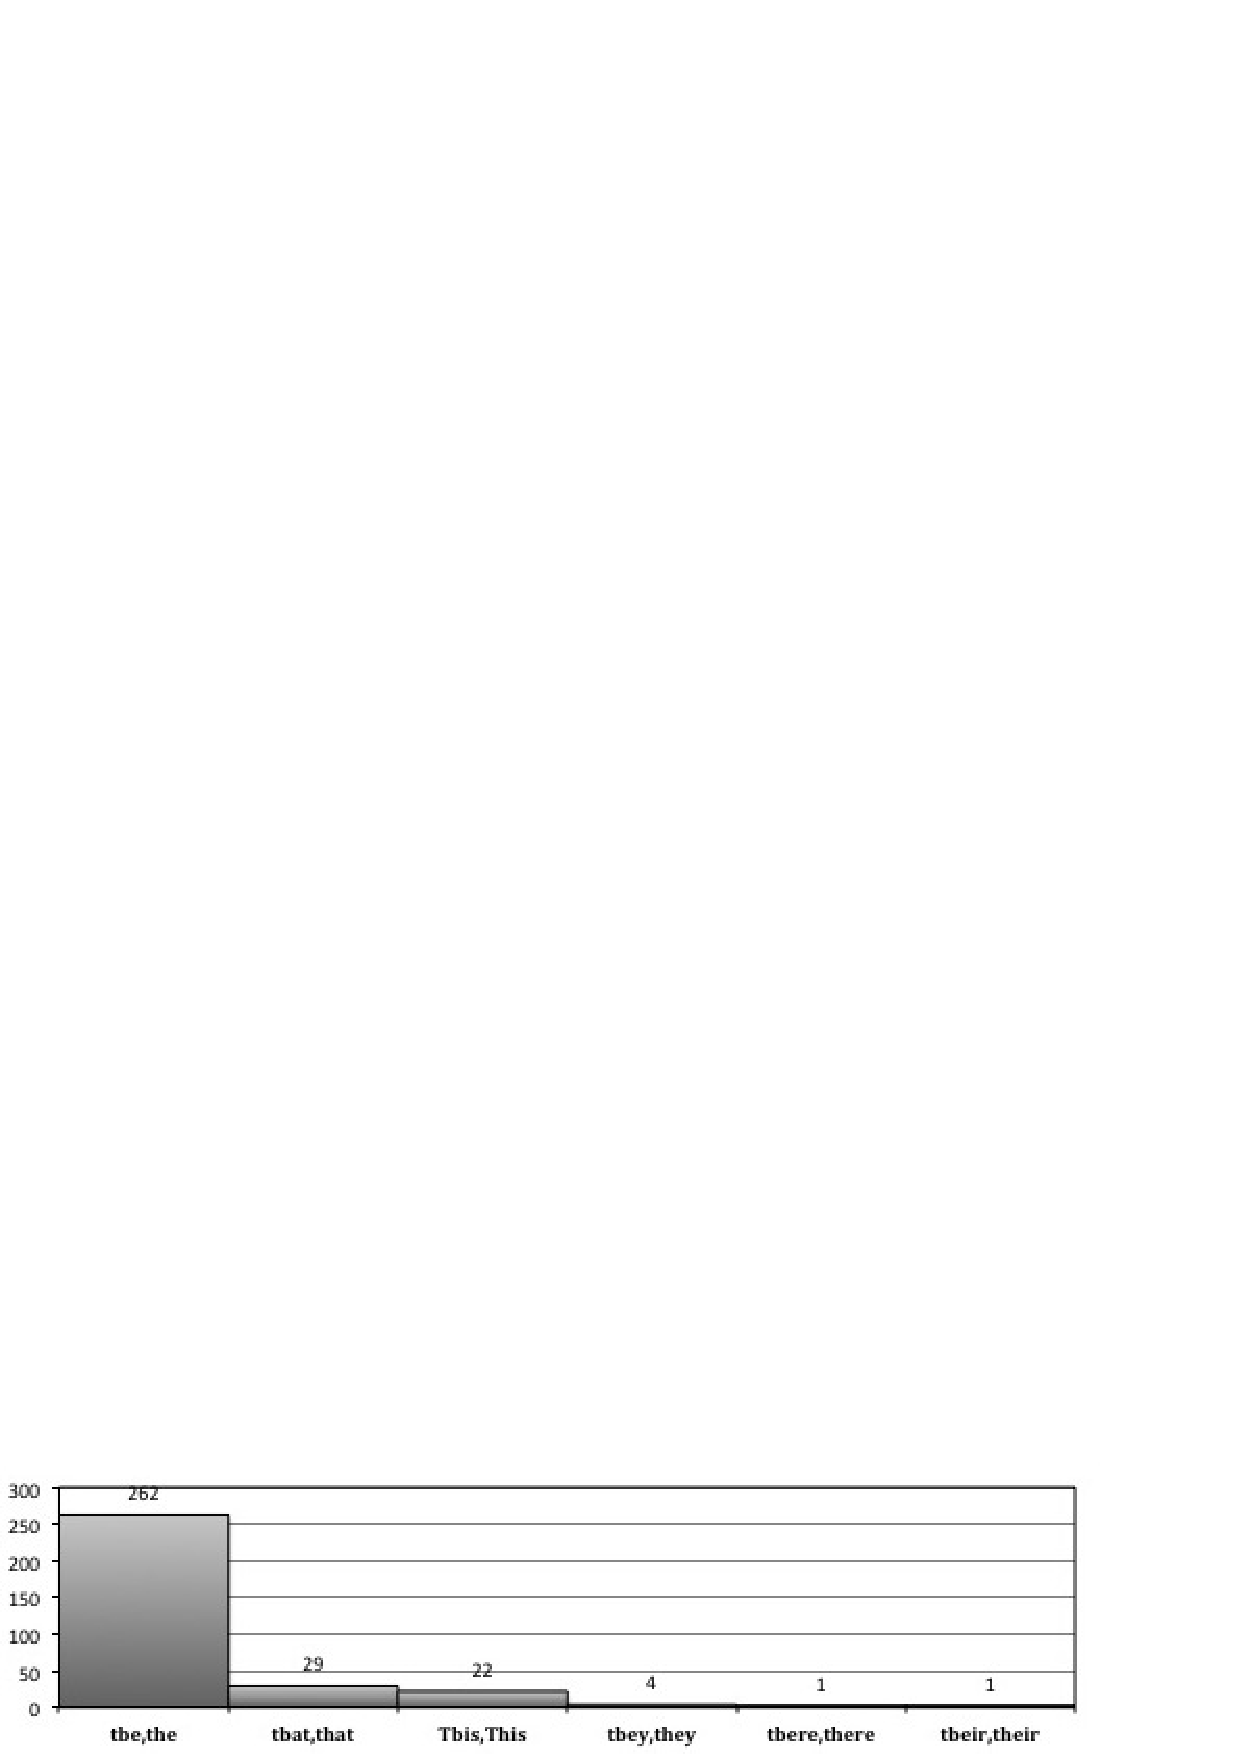
\includegraphics[width=0.45\textwidth,height=0.13\textheight]{./image/stat2copy.jpg}
\label{fig:stat2}
}
%\subfigure[u changed to n]
%{
%%%\includegraphics[width=0.6\columnwidth]{odds_20070813_160000rb_M.pdf}
%\includegraphics[width=0.33\textwidth,height=0.13\textheight]{./image/stat3copy.jpg}
%\label{fig:stat3}
%}
\caption{Example of character level corrections}
\label{News_01}
\end{center}
\end{figure*}


\item \textbf{Model Construction: } The model for classifying crowdsourced text correction is built using a Multiclass Support Vector Machine algorithm \cite{Tsochantaridis_2004}. Each training point belongs to one of $k$ different classes. The goal is to construct a function, which given a new data point, will correctly predict the class to which it belongs.
Different methods have been proposed in literature for solving the SVM multi-class classification problem. Some popular techniques include: a) \textit{One-Versus-All (OVA) classification} Build $k$ different binary classifiers; for the $i^{th}$ classifier, let the positive examples be all points in class $i$ and negative examples not in class $i$. Let $f(x) = \text{arg } max_i f_i(x) $.  b) \textit{one-versus-one} uses the majority voting strategy where each classifier assigns the new instance one of two classes. The class with the majority votes is assigned to the instance.
%%It generates k(k-2)/2 models for a k class problem. This approach is not practical for large-scale classification because of the memory required for storing k(k-1)/2 models.
%c) \textit{Directed Acyclic Graph SVM} in its training phase, it is the same as the one-vs-one method. However, in the testing phase, it uses a rooted binary directed acyclic graph which has k(k-1)/2 internal nodes and k leaves. 
%d) \textit{Error Correcting Output Codes} \cite{multiclassSVM_ecoc} This technique tries to combine binary classifiers by using decorrelations and correct errors.
Crammer and Singer \cite{crammer} pose the multi-class classification problem as a single optimization problem, rather than decomposing it into multiple binary classification problems. A comparison of the above approaches can be found here \cite{comparison}.

For a training set $(x_1,y_1) ... (x_n,y_n)$ with labels $y_i \in \{1, \cdots, k\}$, the multi class problem can be posed as a constrained optimization problem with a quadratic objective function:
$\text{min } \frac{1}{2} \sum_{i = 1}^{k} \parallel w_{i}\parallel^2 + \frac{C}{n} \sum_{i = 1}^{n}\xi_{i} $

s.t. $\forall y \leq k : [x_{1} \cdot w_{yi}] \geq [x_{1} \cdot w_{y}] + 100*\Delta(y_{1},y)-\xi_{1}$
$\cdots$
s.t. $\forall y \leq k : [x_{n} \cdot w_{yn}] \geq [x_{n} \cdot w_{y}] + 100*\Delta(y_{n},y)-\xi_{n}$

Here $C$ is the regularization parameter, $\Delta(y_{j},y), 1 \le j \le n$ is the loss function that returns 0 if $y_{j}$ equals y, and 1 otherwise and $\xi_{i}, 1 \le i \le n$ are the non negative slack variables which measure the degree of misclassification of the instance $x_{i}$. 
%\cite{algo} has to two modules, \textit{svm\_multiclass\_learn} and \textit{svm\_multiclass\_classify}. The learning module learns the model given the parameters and the training data whereas the classification module applies the learned model to the test data to find the error. 
It must be noted that when the data is not linearly separable, the following kernel functions are used for classification:
%the original finite dimensional space is mapped to a much higher dimensional space in order to make the separation easier in that space. The mappings used by SVM schemes are designed to ensure that the dot products may be computed easily in terms of the variables in the original space, by defining them in terms of a Kernel function selected to suit the problem. The types of kernel function used can be described as follows:\\
a) Linear Kernel: $K(x,y) = x^{T}y + c $
b) Polynomial Kernel : $K(x,y) = (\alpha x^{T}y + c)^{d}$
c) Radial Basis Kernel : $K(x,y) = exp(-\lvert \lvert x-y\rvert\rvert^{2}/2\sigma^{2}$)


\begin{table}
\parbox{.55\linewidth}{
\centering
\begin{tabular}{|lllll|}
\hline
C &$AE_{b}$&$AE_{p}$&$AT_{b}$&$AT_{p}$\\
\hline
.0001&99.43$\pm .09$&49.47$\pm0.25$&1.268$\pm.06$&0.11$\pm.01$\\
.1&99.43$\pm .09$&49.464$\pm .47$&2.512$\pm0.01$&0.061$\pm0.01$\\
10&99.43$\pm .09$&4.974$\pm .5$&2.512$\pm0.01$&0.17\\
1000&99.43$\pm .09$&1.743$\pm .14$&3.635$\pm0.08$&0.382$\pm0.04$\\
10000&99.43$\pm .09$&0&6.126$\pm0.02$&0.303$\pm0.02$\\
\hline
\end{tabular}
\caption{Experiment results using linear kernel}
\label{table: error}
}
\hfill
\parbox{.55\linewidth}{
\centering
\begin{tabular}{|l|ll|ll|}
\hline
&Poly&&RBF&\\
\cline{2-5}
C&$AE_{b}$ & $AE_{p}$&$AE_{b}$&$AE_{p}$\\
\hline
.0001&42$\pm.13$&50$\pm.47$&63$\pm.15$&27$\pm.5$\\
100&42$\pm.13$&.33$\pm.2$&63$\pm.16$&3$\pm.4$\\
1000&42$\pm.13$&0$\pm0$&63$\pm.16$&1.7$\pm.2$\\
\hline
C&$AT_{b}$ & $AT_{p}$ &$AT_{b}$ & $AT_{p}$ \\
 \hline
.0001&37$\pm1.4$&10$\pm0.2$&25$\pm0.7$&6$\pm0.2$\\
100&326$\pm11.8$&1239$\pm118$&$540\pm110$&404$\pm34$\\
1000&942$\pm17.4$&764$\pm93$&537$\pm111.72$&957$\pm184$\\
\hline
\end{tabular}
\caption{Experiment Results using polynomial and rbf kernels}
\label{table: kernels}
}
\end{table}



\item \textbf{Information Retrieval Techniques: } The tokens identified by the model as ``spell check",``addition", ``capitalization", and ``punctuation" play an important role in trying to enhance search and retrieval on the archive. This is presented here for the completeness of the architecture, but described in detail in Section~\ref{ir}.

\end{enumerate}


\section{Empirical Evaluation}
\label{sec:evaluation}

The experiments are performed on two machines, one of which is a linux HPC cluster with 20 CPU(s) and 10 cores per socket, 99GB RAM and 2.50GHz of processor speed and the other a dual core mac machine with Intel Core i7 processor, 8GB RAM and 2.9 GHz of processor speed. In these experiments, the regularization parameter $C$ is varied from $0.0001$ to $10000$ for the linear kernel. The performance of the algorithm is evaluated using 10-fold cross validation technique. The \textbf{A}verage loss \textbf{E}rror (AE) and  \textbf{A}verage running \textbf{T}ime (AT) from cross validation for baseline and proposed dataset respectively are represented as $AE_{b}$, $AE_{p}$. Table ~\ref{table: error} shows the result of the experiment, error and running time (cpu seconds) using linear kernel for different values of $C$. Table~\ref{table: kernels} shows the result of the experiment, error and running time (cpu minutes) using polynomial and radial basis kernel.
%The loss is least when the $C = 100$ for the polynomial kernel. However, the time taken to train the model is considerably higher at 106753s. It must also be noted that one can learn less accurate models with linear or RBF kernels faster. Thus, it may be useful to consider a trade-off between accuracy of learnt models versus time taken for classification in large scale deployments.
 
The code used to build the prototype system along with data generated are available from \texttt{https://github.com/megha89/}. It must be noted that the $SVM^{multiclass}$V2.2 package \cite{algo} was used for the implementation of Multi-class SVMs. 
For linear kernels, $SVM^{multiclass}$V2.20 is very fast and runtime scales linearly with the number of training examples. Training of non-linear kernels is very slow using the algorithm described in Section~\ref{arch}.

%\subsection{Results}
%\begin{table}
%\begin{center}
%\begin{tabular}{|lllll|}
%\hline
%C &$AE_{b}$&$AE_{p}$&$AT_{b}$&$AT_{p}$\\
%\hline
%.0001&99.43$\pm .09$&49.47$\pm0.25$&1.268$\pm.06$&0.11$\pm.01$\\
%.1&99.43$\pm .09$&49.464$\pm .47$&2.512$\pm0.01$&0.061$\pm0.01$\\
%10&99.43$\pm .09$&4.974$\pm .5$&2.512$\pm0.01$&0.17\\
%1000&99.43$\pm .09$&1.743$\pm .14$&3.635$\pm0.08$&0.382$\pm0.04$\\
%10000&99.43$\pm .09$&0&6.126$\pm0.02$&0.303$\pm0.02$\\
%\hline
%\end{tabular}
%\caption{Experiment results using linear kernel}
%\label{table: error}
%\end{center}
%\end{table}
%
%\begin{table}[htdp]
%\begin{tabular}{|l|ll|ll|}
%\hline
%&Poly&&RBF&\\
%\cline{2-5}
%C&$AE_{b}$ & $AE_{p}$&$AE_{b}$&$AE_{p}$\\
%\hline
%.0001&42$\pm.13$&50$\pm.47$&63$\pm.15$&27$\pm.5$\\
%100&42$\pm.13$&.33$\pm.2$&63$\pm.16$&3$\pm.4$\\
%1000&42$\pm.13$&0$\pm0$&63$\pm.16$&1.7$\pm.2$\\
%\hline
%C&$AT_{b}$ & $AT_{p}$ &$AT_{b}$ & $AT_{p}$ \\
% \hline
%.0001&37$\pm1.4$&10$\pm0.2$&25$\pm0.7$&6$\pm0.2$\\
%100&326$\pm11.8$&1239$\pm118$&$540\pm110$&404$\pm34$\\
%1000&942$\pm17.4$&764$\pm93$&537$\pm111.72$&957$\pm184$\\
%\hline
%\end{tabular}
%\caption{Experiment Results using polynomial and rbf kernels}
%\label{table: kernels}
%\end{table}


%\subsection{Discussion}
%\subsection{Known Defects}
%The \cite{algo} algorithm converges quickly for linear type kernel but the its performance on test set is poor. For non linear kernels, this algorithm does not scale well for large scale datasets but gives better performance than linear kernels.
\section{Information Retrieval Techniques}
\label{ir}
The following details are relevant: 

\noindent \textbf{Query Set:} To measure the retrieval effectiveness of the corrected text versus the garbled OCR, a list of 20 keywords for search was prepared by randomly sampling from the corrected words.

\noindent \textbf{Software:} PyLucene 3.6.2, a Python extension for accessing Java Apache Lucene was used as an IR software library for enabling full text indexing and search capabilites. Inverted indices are built for both the original and corrected corpus. Keywords from the query set are tested on both corpora and documents containing words in the query set are retrieved. The documents are ranked according to the frequency of the keyword present -- higher the frequency, higher the rank.

\noindent \textbf{Evaluation:} The main aim of this system is to improve the quality of text for use with an IR system. The metric used for evaluation here is mean reciprocal rank (MRR) which produces a list of possible ranked responses to a sample of queries, Q. The reciprocal rank is the multiplicative inverse of the rank of the first correct answer. The first correct answer is decided by the users. The average of the reciprocal ranks over a sample of queries is the mean reciprocal rank.
MRR = $\frac{1}{|Q|} \sum_{i = 1}^{|Q|} \frac{1}{rank_{i}}$

The same set of queries were applied on both the datasets, that is raw OCR and corrected OCR individually. For each of the of $20$ queries, we chose the most relevant document from the retrieved results and observed the rank of the most relevant document in both the set of results. The MRR for the raw OCR data was noted to be $0.355$ whereas for corrected data it was $0.65415$. The higher value of MRR denotes that relevant results get higher priority in corrected corpus.

 
%\noindent \textbf{Evaluation:} The main aim of this system is to improve the quality of text for use with an IR system. The metric used for our evaluation include the standard IR techniques of recall and precision. Recall is defined as the ratio of number of relevant documents returned to the total number of relevant documents for a query, in the collection. Precision is defined as the ratio of number of relevant documents returned to the total number of documents returned for a given query. The document to query relevance is manually determined by other computer science students. The table shows the precision at ten standard recall points for corrected OCR text over the raw OCR text.  

%The metric used to compare the retrieved documents is Spearman's rank correlation coefficient($\rho$). Let $y_{i}$ be the rank ordering of the documents retrieved from the corrected corpus and $x_{i}$ the rank ordering for the garbled text. Let $d_{i}$ = $x_{i}$ - $y_{i}$. Then Spearman's rank correlation $\rho$ is given by: $\rho = 1 - \frac {6\sum d_i^2 }{n(n^2-1)}$.

%\noindent \textbf{Example: } Query word ``Jackson", the evaluation of $\rho$ is shown in Table~\ref{ex}. Here, ${\sum d_i^2}$ = 11 and $\rho$ = 0.45.
%\begin{table}[h]
%\centering
%\begin{tabular}{ l | c | c | c | r | r }
% $Y_{i}$ & $X_{i}$ & $y_{i}$ & $x_{i}$ & $d_{i}$ & $d_{i}^2$ \\
%\hline
%  12-01-1900 & 21-10-1910 & 1 & 10(4) & -3 & 9 \\
%  09-12-1910 & 09-12-1910 & 2 & 2(1) & 0 & 0 \\
%  08-06-1900 & 23-09-1910 & 3 & 7(2) & 1 & 1 \\
%  01-04-1904 & 02-12-1910 & 4 & 8(3) & 1 & 1 \\
%  25-05-1900 & 23-12-1910 & 5 & 11(5) & 0 & 0 \\
%\end{tabular}
%\label{ex}
%\end{table}

\noindent \textbf{Deployment: }The full-scale deployment of this prototype system is being considered on old historic newspaper archives at California Digital Newspaper Collection and the New York Public Library among others, where  user text corrections are used extensively for cleaning garbled OCR. 

\section{Related Work}
\label{sec:related}
\noindent \textbf{Optical Character Recognition (OCR)} is a commonly used method of digitizing printed texts so that it can be searched and displayed online, stored compactly and used in text mining applications. The text generated from OCR devices is often garbled due to variations in quality of the input paper, size and style of the font and column layout, its condition at the time of microfilming, choice of scanner, and the quality of the OCR software. Several techniques for post processing garbled OCR have been designed \cite{Fujisawa_08}, \cite{Esakov_94}, \cite{Lecun_90}. These include:

\noindent \textbf{Dictionary based schemes: }These algorithms use a dictionary to spellcheck misspelled OCR recognized words. They correct non-word errors - words that are recognized by the OCR device but do not correspond to any entry in the lexicon. Niwa et al. \cite{postprocessing} proposed an OCR post error correction method based on pattern learning where a list of suitable candidates is generated from the lexicon and the best candidate is selected as a correction. Yannakoudakis and Fawthrop \cite{Yannakoudakis_83} conducted a study to create a set of rules based on common misspelling pattern and used them to correct errors. Cherkassky and Vassilas \cite{Cherkassky_89} use back propagation algorithms for correction. 
%\cite{statistical} proposed using Hidden Markov Models (HMMs) to integrate syntactic information into the post-processing error correction. 
%The suggested model achieved a higher rate of error correction due to its statistical nature in selecting the most probable candidate for a particular misspelled word.

\noindent \textbf{Context based schemes: }These algorithms perform error detection and correction based on the grammatical error and semantic context. They are able to correct real-word errors -- words that are recognized by the OCR system and correspond to an entry in the lexicon. Tong and Evans \cite{Tong96astatistical} describe an automatic, context-sensitive, word-error correction system based on Statistical Language Modeling (SLM). The system exploits information from letter n-grams, character confusion probabilities and word bi-gram probabilities. Golding et al. \cite{contextbased} applies a part-of-speech (POS) tagger enhanced by word trigram model and a statistical Bayesian classifier to correct real-word errors in OCR text. Reynaert \cite{Reynaert2008a} presents a system for reducing the level of OCR-induced typographical variation in large text collections called Text-Induced Corpus Clean-up (TICCL). The system focuses on high-frequency words to be cleaned and gathers all typographical variants for any particular focus word that lie within the predefined Levenshtein distance. Bassil et al. \cite{Bassil_12a,Bassil_12b} propose a post-processing context-based error correction algorithm for detecting and correcting OCR non-word and real-word errors. The proposed algorithm is based on Google's online spelling suggestion. Abdulkader et al. \cite{lowcost}  present a method for digitizing textual data by using neural network classifiers to estimate OCR errors, clustering similar errors, designing a user interface and using active learning to tune the error estimation from user labeled data. 
Velagapudi \cite{velagapudi} uses a combination of classifiers -- kNN classifier,  multilayer perceptrons and SVM to discuss the effects of error correction on the classification accuracy of each method. 

Very little work has been done on automatic \emph{classification} of OCR error corrections\footnote{Most prior work has dealt with evaluation of candidate corrections for OCR errors.} to get a clear understanding of the \emph{nature} of errors encountered -- Esakov et al. \cite{Esakov_94a} suggest classification of output from the OCR engine as simple substitutions ($e \rightarrow c$), improper segmentation or multiple substitutions $(T \rightarrow 'l, m \rightarrow rn, he \rightarrow b)$, deletions and insertions (involving space) and unrecognized characters $(u \rightarrow \sim)$. They use a new variant of the dynamic programming algorithm for classification. In \cite{hybred}, OCR documents are classified into fixed number of categories based on their content. The accuracy of their approach was best when evaluated using SVM among other algorithms. Daoason \cite{Jon_12} posits that OCR errors are not random -- for example, it is extremely unlikely that the letter $o$ will be misrecognized as $x$ since they are very dissimilar. He classifies OCR errors as character errors (characters in the input document that are replaced with other characters), word errors (word in the input document is not correct or not present in the OCR generated text), or zoning errors (OCR software is unable to decipher zones correctly). Our work primarily focusses on \emph{manual} error correction classification where the task of correcting OCR errors is outsourced to a crowd of workers. 
%By engaging a large crowd of people for ideas, skills or participation the quality of work done is superior and relatively inexpensive.

%It is estimated that the total count of published books in the world is around 130 million \cite{bookscount}. Many of these books published are only available in printed format due to reasons like copyright and licensing issues. This limits the search of these articles, their availability and accessibility on the web. As of 2013, more than 30 million books have been digitised by Google Books Library Project \cite{gblp}. It uses reCAPTCHA to digitise books one word at a time by sending words that can not be read by the computer to the web in the form of CAPTCHAs for humans to decipher \cite{recaptcha}. 

%The OCR enables searching of full text data but it is not 100\% accurate. Its accuracy largely depends on paper quality of the original issue, font style, column layouts, its condition at the time of microfilming, choice of scanner \cite{issue}, and the quality of the OCR software. The OCR errors are widely classified as non-word errors and real-word errors. A non-word error takes place when the erroneous word is not a dictionary word whereas in real-word error the erroneous word is correctly spelt and therefore can be found in the dictionary but incorrectly used in context.
%The error generated by OCR can be classified in several categories. One such classification similar to ours is done by \cite{post-correction}. It gives an exhaustive error classification that helps in classifying real words , that is words that are not contained in any of the dictionary, e.g. names, out-dated or historic spelling variations. Segmentation errors, Hyphenation error, Misrecognition of characters, Punctuation errors, Case sensitivity, Changed word meaning are the classes required for better classification of OCR errors.

%The OCR errors are usually dependent on some major factors like the page quality, text layout, font styles. In \mydoubleq{Issues in automatic error correction}, the experimental analysis has shown that there is another important factor that impacts the performance of the OCR errors which is the choice of scanners used to scan the printed text. The type of scanner used not only affect the quantity of errors but quality as well. Their algorithm for classifying OCR errors is based minimising the cost of basic operations used to transform one string to another, also known as edit distance using dynamic programming approach.\\
%\mydoubleq{Unsupervised Post Correction} paper talks about the post processing of OCR text to minimise the errors. It uses a combination of Anagram Hashing techniques, bigram approach on word level to consider the context and a  similarity key technique called OCR-key.  Anagram Hashing technique uses a hashing function that assigns same number to all those words that have same characters. OCR key observes the shape of characters to know the nature of OCR system and its generated errors.
\noindent \textbf{Crowdsourced OCR correction }Recruiting users and paying them small sums of money to tag and annotate text and images in large digital archives has become common practice (e.g. Amazon's Mechanical Turk, reCAPTCHA \cite{vonAhn_08}, ESP \cite{vonAhn_04}) and Games with a Purpose \cite{Ahn_08w}. A number of recent papers have evaluated the effectiveness of using Mechanical Turk to create annotated data for text and natural language processing applications \cite{Snow_08}. In the same vein, many workshops and conferences have been organized on the theme of machine learning in human computation, crowdsourcing and collective intelligence\footnote{See http://ir.ischool.utexas.edu/crowd/}. 

Intuitively, the easiest way to correct garbled OCR text is to hire a group of people to edit it manually. Distributed Proofreaders (DP) \cite{DP} is a web-based project designed to facilitate proofreading of paper books into e-books and was meant to assist the project Gutenberg\footnote{http://www.gutenberg.org/}. Wikipedia is yet another example of a large scale crowdsourcing project. Yamangil et al. \cite{wikiedits} proposed a learning algorithm for mining wikipedia edit history using baseline Hidden Markov Model augmented with perceptron re-ranking. The model was trained on wikipedia edits and hence incorporated human corrections. 
%\subsection{Multi-class SVM}



\section{Conclusion \& Future Work}
\label{sec:conc}
The California Digital Newspaper Collection has an archive of 400,000 pages of historical California newspapers published between 1846 to 1922. This archive which has been subjected to OCR and is currently stored in an online database making them accessible to patrons. The OCR scanning process generates lot of garbled text which needs to be corrected to make the online newspaper repository more accessible to general public. 

In this paper, we present a system for Classification of Crowdsourced Text Correction which is capable of modelling user corrections using state-of-the-art machine learning techniques and retrieve categories which are likely to enhance search on the archive such as addition of words, elimination of typographical errors or addition of content. Information retrieval metric, mean reciprocal rank is used to quantify the effectiveness of the user text correction. The prototype system is being considered for deployment on historic newspaper archives at the California Digital Newspaper Collection and the New York Public Library.

% use section* for acknowledgement
\section*{Acknowledgment}
This work is supported by funding from the National Endowment for Humanities, Grant No: NEH HD-51153-10. The authors would like to thank Stefan Boddie, DL Consulting, Ltd., New Zealand for sharing experiences with the Veridian software and Luis. C. Baquera, University of California, Riverside for providing data generated from the log files at CDNC.\\

%\section{Empirical Evaluation}
%\label{sec:evaluation}
%
%Experiments are performed by randomly selecting $70\%$ of the data\footnote{Approximately 30,815 instances}  as the train set. For each experiment, the regularization parameter $C$ and the type of kernel $t$ are varied as $0.001,0.01,0.1,1,10,100$ and Linear, Polynomial and Radial Basis Function kernel respectively. The experiments are performed on two machines, one of which is a linux server and the other a dual core Mac machine with Intel Core i7 processor, 8GB RAM, 2.9 GHz of processor speed. Each experiment is repeated $5$ times and the average loss on the test set and CPU runtime are reported. Table ~\ref{table: error} presents the average loss on test set for different values of $C$ and $t$; $AE_{L}$, $AE_{P}$, $AE_{R}$ represents the average loss on the linear, polynomial and RBF kernels respectively. Table ~\ref{table: runtime} shows the average runtime (cpu sec) required to learn a model for various values of $C$ and for different kernels. Here, $AT_{L}$, $AT_{P}$, $AT_{R}$ refers to the average run time of linear, polynomial and rbf kernels respectively. The loss is least when the $C = 100$ for the polynomial kernel. However, the time taken to train the model is considerably higher at 106753s. It must also be noted that one can learn less accurate models with linear or RBF kernels faster. Thus, it may be useful to consider a trade-off between accuracy of learnt models versus time taken for classification in large scale deployments.
% 
%The code used to build the prototype system along with data generated are available from \texttt{https://github.com/megha89/}. It must be noted that the $SVM^{multiclass}$V2.2 package \cite{algo} was used for the implementation of Multi-class SVMs. 
%For linear kernels, $SVM^{multiclass}$V2.20 is very fast and runtime scales linearly with the number of training examples. Training of non-linear kernels is very slow using the algorithm described in Section~\ref{arch}.
%
%%\subsection{Results}
%
%\begin{table}[htdp]
%\begin{center}
%\begin{tabular}{| c | c | c | c |}
%\hline
%C & $AE_{L}$ & $AE_{P}$ & $AE_{R}$ \\
%\hline
%.001 & 32.06 $\pm$0.149  & 32.06$\pm$0.149 & 11.96$\pm$0.101 \\
%.01 & 32.06$\pm$0.149 & 32.06$\pm$0.149 & 12.04$\pm$0.199 \\
%.1 & 32.06$\pm$0.149 & 29.10$\pm$0.133  & 12.04$\pm$0.199  \\
%1 &29.10$\pm$0.133  & 28.99$\pm$0.264  & 6.36$\pm$0.142  \\
%10 & 29.20$\pm$0.133 & 8.338$\pm$0.107 & 6.36$\pm$0.142 \\
%100 & 29.20$\pm$0.133 & 0.58$\pm.034$ & 6.35$\pm0.16$  \\
%\hline
%\end{tabular}
%\end{center}
%\caption{Experiment Results : Average loss error (test set)}
%\label{table: error}
%\end{table}
%
%
%\begin{table}[htdp]
%\begin{center}
%\begin{tabular}{| l | c | c | l |}
%\hline
%C & $ AT_{L} $ & $AT_{P}$ & $AT_{R}$ \\
%\hline
%.001 & 0.218 & 5192 & 4596 \\
%.01 & 0.202 & 5166 & 4460 \\
%.1 & 0.208 & 72225 & 4377 \\
%1 & 0.678 & 81251 & 16468 \\
%10 & 0.672 & 260316 & 55308 \\
%100 & 0.998 & 106753  & 48734  \\
%\hline
%\end{tabular}
%\end{center}
%\caption{Experiment Results : Training time (cpu sec)}
%\label{table: runtime}
%\end{table}
%
%%\subsection{Discussion}
%
%%\subsection{Known Defects}
%%The \cite{algo} algorithm converges quickly for linear type kernel but the its performance on test set is poor. For non linear kernels, this algorithm does not scale well for large scale datasets but gives better performance than linear kernels.
%
%\section{Information Retrieval Techniques}
%\label{ir}
%The following details are relevant: 
%
%\noindent \textbf{Query Set:} To measure the retrieval effectiveness of the corrected text versus the garbled OCR, a list of 60 keywords for search was prepared by randomly sampling from the corrected words.
%
%\noindent \textbf{Software:} PyLucene 3.6.2, a Python extension for accessing Java Apache Lucene was used as an IR software library for enabling full text indexing and search capabilites. Inverted indices are built for both the original and corrected corpus. Keywords from the query set are tested on both corpora and documents containing words in the query set are retrieved. The documents are ranked according to the frequency of the keyword present -- higher the frequency, higher the rank.
% 
%\noindent \textbf{Evaluation:} The main aim of this system is to improve the quality of text for use with an IR system. The metric used for our evaluation include the standard IR techniques of recall and precision. Recall is defined as the ratio of number of relevant documents returned to the total number of relevant documents for a query, in the collection. Precision is defined as the ratio of number of relevant documents returned to the total number of documents returned for a given query. The document to query relevance is manually determined by other computer science students. The table shows the precision at ten standard recall points for corrected OCR text over the raw OCR text.  
%
%%The metric used to compare the retrieved documents is Spearman's rank correlation coefficient($\rho$). Let $y_{i}$ be the rank ordering of the documents retrieved from the corrected corpus and $x_{i}$ the rank ordering for the garbled text. Let $d_{i}$ = $x_{i}$ - $y_{i}$. Then Spearman's rank correlation $\rho$ is given by: $\rho = 1 - \frac {6\sum d_i^2 }{n(n^2-1)}$.
%
%%\noindent \textbf{Example: } Query word ``Jackson", the evaluation of $\rho$ is shown in Table~\ref{ex}. Here, ${\sum d_i^2}$ = 11 and $\rho$ = 0.45.
%%\begin{table}[h]
%%\centering
%%\begin{tabular}{ l | c | c | c | r | r }
%% $Y_{i}$ & $X_{i}$ & $y_{i}$ & $x_{i}$ & $d_{i}$ & $d_{i}^2$ \\
%%\hline
%%  12-01-1900 & 21-10-1910 & 1 & 10(4) & -3 & 9 \\
%%  09-12-1910 & 09-12-1910 & 2 & 2(1) & 0 & 0 \\
%%  08-06-1900 & 23-09-1910 & 3 & 7(2) & 1 & 1 \\
%%  01-04-1904 & 02-12-1910 & 4 & 8(3) & 1 & 1 \\
%%  25-05-1900 & 23-12-1910 & 5 & 11(5) & 0 & 0 \\
%%\end{tabular}
%%\label{ex}
%%\end{table}
%
%\noindent \textbf{Deployment: }The full-scale deployment of this prototype system is being considered on old historic newspaper archives at California Digital Newspaper Collection and the New York Public Library among others, where  user text corrections are used extensively for cleaning garbled OCR. 
%
%\section{Related Work}
%\label{sec:related}
%\noindent \textbf{Optical Character Recognition (OCR)} is a commonly used method of digitizing printed texts so that it can be searched and displayed online, stored compactly and used in text mining applications. The text generated from OCR devices is often garbled due to variations in quality of the input paper, size and style of the font and column layout, its condition at the time of microfilming, choice of scanner, and the quality of the OCR software. Several techniques for post processing garbled OCR have been designed \cite{Fujisawa_08}, \cite{Esakov_94}, \cite{Lecun_90}. These include:
%
%\noindent \textbf{Dictionary based schemes: }These algorithms use a dictionary to spellcheck misspelled OCR recognized words. They correct non-word errors - words that are recognized by the OCR device but do not correspond to any entry in the lexicon. Niwa et al. \cite{postprocessing} proposed an OCR post error correction method based on pattern learning where a list of suitable candidates is generated from the lexicon and the best candidate is selected as a correction. Yannakoudakis and Fawthrop \cite{Yannakoudakis_83} conducted a study to create a set of rules based on common misspelling pattern and used them to correct errors. Cherkassky and Vassilas \cite{Cherkassky_89} use back propagation algorithms for correction. 
%%\cite{statistical} proposed using Hidden Markov Models (HMMs) to integrate syntactic information into the post-processing error correction. 
%%The suggested model achieved a higher rate of error correction due to its statistical nature in selecting the most probable candidate for a particular misspelled word.
%
%\noindent \textbf{Context based schemes: }These algorithms perform error detection and correction based on the grammatical error and semantic context. They are able to correct real-word errors -- words that are recognized by the OCR system and correspond to an entry in the lexicon. Tong and Evans \cite{Tong96astatistical} describe an automatic, context-sensitive, word-error correction system based on Statistical Language Modeling (SLM). The system exploits information from letter n-grams, character confusion probabilities and word bi-gram probabilities. Golding et al. \cite{contextbased} applies a part-of-speech (POS) tagger enhanced by word trigram model and a statistical Bayesian classifier to correct real-word errors in OCR text. Reynaert \cite{Reynaert2008a} presents a system for reducing the level of OCR-induced typographical variation in large text collections called Text-Induced Corpus Clean-up (TICCL). The system focuses on high-frequency words to be cleaned and gathers all typographical variants for any particular focus word that lie within the predefined Levenshtein distance. Bassil et al. \cite{Bassil_12a,Bassil_12b} propose a post-processing context-based error correction algorithm for detecting and correcting OCR non-word and real-word errors. The proposed algorithm is based on Google's online spelling suggestion. Abdulkader et al. \cite{lowcost}  present a method for digitizing textual data by using neural network classifiers to estimate OCR errors, clustering similar errors, designing a user interface and using active learning to tune the error estimation from user labeled data. 
%Velagapudi \cite{velagapudi} uses a combination of classifiers -- kNN classifier,  multilayer perceptrons and SVM to discuss the effects of error correction on the classification accuracy of each method. 
%
%Very little work has been done on automatic \emph{classification} of OCR error corrections\footnote{Most prior work has dealt with evaluation of candidate corrections for OCR errors.} to get a clear understanding of the \emph{nature} of errors encountered -- Esakov et al. \cite{Esakov_94a} suggest classification of output from the OCR engine as simple substitutions ($e \rightarrow c$), improper segmentation or multiple substitutions $(T \rightarrow 'l, m \rightarrow rn, he \rightarrow b)$, deletions and insertions (involving space) and unrecognized characters $(u \rightarrow \sim)$. They use a new variant of the dynamic programming algorithm for classification. In \cite{hybred}, OCR documents are classified into fixed number of categories based on their content. The accuracy of their approach was best when evaluated using SVM among other algorithms. Daoason \cite{Jon_12} posits that OCR errors are not random -- for example, it is extremely unlikely that the letter $o$ will be misrecognized as $x$ since they are very dissimilar. He classifies OCR errors as character errors (characters in the input document that are replaced with other characters), word errors (word in the input document is not correct or not present in the OCR generated text), or zoning errors (OCR software is unable to decipher zones correctly). Our work primarily focusses on \emph{manual} error correction classification where the task of correcting OCR errors is outsourced to a crowd of workers. 
%%By engaging a large crowd of people for ideas, skills or participation the quality of work done is superior and relatively inexpensive.
%
%%It is estimated that the total count of published books in the world is around 130 million \cite{bookscount}. Many of these books published are only available in printed format due to reasons like copyright and licensing issues. This limits the search of these articles, their availability and accessibility on the web. As of 2013, more than 30 million books have been digitised by Google Books Library Project \cite{gblp}. It uses reCAPTCHA to digitise books one word at a time by sending words that can not be read by the computer to the web in the form of CAPTCHAs for humans to decipher \cite{recaptcha}. 
%
%%The OCR enables searching of full text data but it is not 100\% accurate. Its accuracy largely depends on paper quality of the original issue, font style, column layouts, its condition at the time of microfilming, choice of scanner \cite{issue}, and the quality of the OCR software. The OCR errors are widely classified as non-word errors and real-word errors. A non-word error takes place when the erroneous word is not a dictionary word whereas in real-word error the erroneous word is correctly spelt and therefore can be found in the dictionary but incorrectly used in context.
%%The error generated by OCR can be classified in several categories. One such classification similar to ours is done by \cite{post-correction}. It gives an exhaustive error classification that helps in classifying real words , that is words that are not contained in any of the dictionary, e.g. names, out-dated or historic spelling variations. Segmentation errors, Hyphenation error, Misrecognition of characters, Punctuation errors, Case sensitivity, Changed word meaning are the classes required for better classification of OCR errors.
%
%%The OCR errors are usually dependent on some major factors like the page quality, text layout, font styles. In \mydoubleq{Issues in automatic error correction}, the experimental analysis has shown that there is another important factor that impacts the performance of the OCR errors which is the choice of scanners used to scan the printed text. The type of scanner used not only affect the quantity of errors but quality as well. Their algorithm for classifying OCR errors is based minimising the cost of basic operations used to transform one string to another, also known as edit distance using dynamic programming approach.\\
%%\mydoubleq{Unsupervised Post Correction} paper talks about the post processing of OCR text to minimise the errors. It uses a combination of Anagram Hashing techniques, bigram approach on word level to consider the context and a  similarity key technique called OCR-key.  Anagram Hashing technique uses a hashing function that assigns same number to all those words that have same characters. OCR key observes the shape of characters to know the nature of OCR system and its generated errors.
%\noindent \textbf{Crowdsourced OCR correction }Recruiting users and paying them small sums of money to tag and annotate text and images in large digital archives has become common practice (e.g. Amazon's Mechanical Turk, reCAPTCHA \cite{vonAhn_08}, ESP \cite{vonAhn_04}) and Games with a Purpose \cite{Ahn_08w}. A number of recent papers have evaluated the effectiveness of using Mechanical Turk to create annotated data for text and natural language processing applications \cite{Snow_08}. In the same vein, many workshops and conferences have been organized on the theme of machine learning in human computation, crowdsourcing and collective intelligence\footnote{See http://ir.ischool.utexas.edu/crowd/}. 
%
%Intuitively, the easiest way to correct garbled OCR text is to hire a group of people to edit it manually. Distributed Proofreaders (DP) \cite{DP} is a web-based project designed to facilitate proofreading of paper books into e-books and was meant to assist the project Gutenberg\footnote{http://www.gutenberg.org/}. Wikipedia is yet another example of a large scale crowdsourcing project. Yamangil et al. \cite{wikiedits} proposed a learning algorithm for mining wikipedia edit history using baseline Hidden Markov Model augmented with perceptron re-ranking. The model was trained on wikipedia edits and hence incorporated human corrections. 
%%\subsection{Multi-class SVM}
%
%
%
%\section{Conclusion \& Future Work}
%\label{sec:conc}
%The California Digital Newspaper Collection has an archive of 400,000 pages of historical California newspapers published between 1846 to 1922. This archive which has been subjected to OCR and is currently stored in an online database making them accessible to patrons. The OCR scanning process generates lot of garbled text which needs to be corrected to make the online newspaper repository more accessible to general public. 
%
%In this paper, we present a system for Classification of Crowdsourced Text Correction which is capable of modeling user corrections using state-of-the-art machine learning techniques and retrieve categories which are likely to enhance search on the archive such as addition of words, elimination of typographical errors or addition of content. Information retrieval metrics are used to quantify the effectiveness of the user text correction. The prototype system is being considered for deployment on historic newspaper archives at the California Digital Newspaper Collection and the New York Public Library.
%
%% use section* for acknowledgement
%\section*{Acknowledgment}
%This work is supported by funding from the National Endowment for Humanities, Grant No: NEH HD-51153-10. The authors would like to thank Stefan Boddie, DL Consulting, Ltd., New Zealand for sharing experiences with the Veridian software and Luis. C. Baquera, University of California, Riverside for providing data generated from the log files at CDNC.\\


\bibliographystyle{IEEEtran}
\bibliography{ictaiPaper}
\end{document}

%\begin{thebibliography}{1}
%
%\bibitem{IEEEhowto:kopka}
%H.~Kopka and P.~W. Daly, \emph{A Guide to \LaTeX}, 3rd~ed.\hskip 1em plus
%  0.5em minus 0.4em\relax Harlow, England: Addison-Wesley, 1999.
%
%\end{thebibliography}
%
%
%
%
%% that's all folks
%\end{document}






% An example of a floating figure using the graphicx package.
% Note that \label must occur AFTER (or within) \caption.
% For figures, \caption should occur after the \includegraphics.
% Note that IEEEtran v1.7 and later has special internal code that
% is designed to preserve the operation of \label within \caption
% even when the captionsoff option is in effect. However, because
% of issues like this, it may be the safest practice to put all your
% \label just after \caption rather than within \caption{}.
%
% Reminder: the "draftcls" or "draftclsnofoot", not "draft", class
% option should be used if it is desired that the figures are to be
% displayed while in draft mode.
%
%\begin{figure}[!t]
%\centering
%\includegraphics[width=2.5in]{myfigure}
% where an .eps filename suffix will be assumed under latex, 
% and a .pdf suffix will be assumed for pdflatex; or what has been declared
% via \DeclareGraphicsExtensions.
%\caption{Simulation Results}
%\label{fig_sim}
%\end{figure}

% Note that IEEE typically puts floats only at the top, even when this
% results in a large percentage of a column being occupied by floats.


% An example of a double column floating figure using two subfigures.
% (The subfig.sty package must be loaded for this to work.)
% The subfigure \label commands are set within each subfloat command, the
% \label for the overall figure must come after \caption.
% \hfil must be used as a separator to get equal spacing.
% The subfigure.sty package works much the same way, except \subfigure is
% used instead of \subfloat.
%
%\begin{figure*}[!t]
%\centerline{\subfloat[Case I]\includegraphics[width=2.5in]{subfigcase1}%
%\label{fig_first_case}}
%\hfil
%\subfloat[Case II]{\includegraphics[width=2.5in]{subfigcase2}%
%\label{fig_second_case}}}
%\caption{Simulation results}
%\label{fig_sim}
%\end{figure*}
%
% Note that often IEEE papers with subfigures do not employ subfigure
% captions (using the optional argument to \subfloat), but instead will
% reference/describe all of them (a), (b), etc., within the main caption.


% An example of a floating table. Note that, for IEEE style tables, the 
% \caption command should come BEFORE the table. Table text will default to
% \footnotesize as IEEE normally uses this smaller font for tables.
% The \label must come after \caption as always.
%
%\begin{table}[!t]
%% increase table row spacing, adjust to taste
%\renewcommand{\arraystretch}{1.3}
% if using array.sty, it might be a good idea to tweak the value of
% \extrarowheight as needed to properly center the text within the cells
%\caption{An Example of a Table}
%\label{table_example}
%\centering
%% Some packages, such as MDW tools, offer better commands for making tables
%% than the plain LaTeX2e tabular which is used here.
%\begin{tabular}{|c||c|}
%\hline
%One & Two\\
%\hline
%Three & Four\\
%\hline
%\end{tabular}
%\end{table}


% Note that IEEE does not put floats in the very first column - or typically
% anywhere on the first page for that matter. Also, in-text middle ("here")
% positioning is not used. Most IEEE journals/conferences use top floats
% exclusively. Note that, LaTeX2e, unlike IEEE journals/conferences, places
% footnotes above bottom floats. This can be corrected via the \fnbelowfloat
% command of the stfloats package.


% conference papers do not normally have an appendix


% use section* for acknowledgement
%\section*{Acknowledgment}
%
%
%The authors would like to thank...
%more thanks here


% trigger a \newpage just before the given reference
% number - used to balance the columns on the last page
% adjust value as needed - may need to be readjusted if
% the document is modified later
%\IEEEtriggeratref{8}
% The "triggered" command can be changed if desired:
%\IEEEtriggercmd{\enlargethispage{-5in}}

% references section

% can use a bibliography generated by BibTeX as a .bbl file
% BibTeX documentation can be easily obtained at:
% http://www.ctan.org/tex-archive/biblio/bibtex/contrib/doc/
% The IEEEtran BibTeX style support page is at:
% http://www.michaelshell.org/tex/ieeetran/bibtex/
%\bibliographystyle{IEEEtran}
% argument is your BibTeX string definitions and bibliography database(s)
%\bibliography{IEEEabrv,../bib/paper}
%
% <OR> manually copy in the resultant .bbl file
% set second argument of \begin to the number of references
% (used to reserve space for the reference number labels box)
%\begin{thebibliography}{1}
%
%\bibitem{IEEEhowto:kopka}
%H.~Kopka and P.~W. Daly, \emph{A Guide to \LaTeX}, 3rd~ed.\hskip 1em plus
%  0.5em minus 0.4em\relax Harlow, England: Addison-Wesley, 1999.
%
%\end{thebibliography}
%
%
%
%
%% that's all folks
%\end{document}


